\documentclass[DM,lsstdraft,toc]{lsstdoc}
\usepackage{graphicx}
\usepackage{url}
\usepackage{color}

\title[Photo-$z$ for LSST Objects]{A Roadmap to Photometric Redshifts for the LSST {\tt Object} Catalog}

\author{M.~L.~Graham, J.~Bosch, L.~P.~Guy, \\ and the DM System Science Team.}

\setDocRef{DMTN-049}
\date{\today}
\setDocRevision{TBD} 
\setDocStatus{draft}

\setDocAbstract{
This roadmap guides the Rubin Observatory Data Management (DM) team's efforts to engage with the scientific community of data-rights holders in order to validate and implement one or more existing photometric redshift (photo-$z$) estimators into the Data Release (DR) processing pipeline, and serve the resulting photo-$z$ data products for the first DR {\tt Object} catalog (and beyond).

\medskip
The DM-generated photo-$z$ estimates will initially be a {\it minimum scientifically-viable product} that serves the {\it widest variety of science applications}.
One or more {\it existing, community-vetted algorithms} will be adopted; this selection will be subject to constraints imposed by the DM System (e.g., compute resources). 

\medskip
The Rubin science community has a considerable wealth of expertise in generating photo-$z$ catalogs and will be the primary users of the DR {\tt Object} catalog photo-$z$ data products.
Thus, the processes to define the estimator(s) minimum attributes, selection criteria, and validation metrics, and to scientifically validate the estimator(s) with commissioning data, will be a joint community-project venture.

\medskip
This roadmap is a \textit{\textbf{living document}} to guide these processes, and it will evolve over time to incorporate input from the science community.
DM's activities in this regard are divided into three phases:
\begin{itemize}
\item {\bf Phase 1:} Define the initial minimum scientific attributes and selection criteria for photo-$z$ estimators (\S~\ref{sec:mvp} \& \ref{sec:eval}) by soliciting community input regarding their science needs and interests. (End: Aug 31 2021).
\item {\bf Phase 2:} Solicit formal community "letters of recommendation" regarding photo-$z$ estimators (\S~\ref{sec:lor}; due: Apr 31 2022) in order to generate a shortlist of community-vetted photo-$z$ estimator(s) to use for Phase 3.
\item {\bf Phase 3:} Facilitate community participation in a "Photo-$z$ Validation Cooperative" based on commissioning data (\S~\ref{sec:pzcoop}), which will inform DM's selection of community-vetted photo-$z$ estimator(s) for DR1. (Dates to be determined).
\end{itemize}

This roadmap includes in-kind contributions from international partnerships to {\tt Object} catalog photo-$z$ for DR1 and beyond, as well as potential processes of improving and evolving the DR {\tt Object} catalog photo-$z$ and/or of ingesting and federating user-generated photo-$z$ catalogs during Operations.
}

\setDocChangeRecord{%
\addtohist{1}{2017-04-01}{Initial release of preliminary investigation.}{Melissa Graham}
\addtohist{2}{2018-10-16}{Edited to align with recent DPDD updates, some of which were based on the recommendations of Version 1 of this document.}{Melissa Graham}
\addtohist{3}{2020-XX-XX}{Updated as per Jira ticket DM-6367. Included community input, and revised to be a roadmap for future community engagement.}{Melissa Graham}
}

\begin{document}

\maketitle

% CITATION EXAMPLES
%\verb|\citellp|: \citellp{LPM-17, LSE-30} \\
%\verb|\citell|: (SRD; \citell{LPM-17,LSE-29}) \\
%\verb|\citep[][]|: \citep[e.g.,][are interesting]{LPM-17,LSE-29} \\
%\verb|\cite|: \cite{LPM-17,LSE-29} \\
%\citet{2018A&C....25...58G} \\     % Gschwend et al. [13]
%\citep{2018A&C....25...58G} \\    % [13]
%\citealt{2018A&C....25...58G} \\   % Gschwend et al. 13



% % % % % % % % % % % % % % % % % % % % % % % % % % % % % %
\section{Introduction} \label{sec:intro}

A {\it photometric redshift} is an estimate of an object's cosmological redshift which is based on its photometry (e.g., apparent magnitudes in multiple filters) instead of on its spectral features (e.g., emission and absorption lines). 
Redshift is a key component of many science goals that will be pursued with data from the Legacy Survey of Space and Time (LSST).
Since it will be impossible to obtain spectra for the billions of galaxies that LSST will observe, photometric redshift estimates will be necessary.

Typically, photometric redshift estimators either fit template spectra to the observed photometry or match photometry to a training set of galaxies with spectroscopic redshifts. 
The latter is often done with machine learning codes, and hybrid photo-$z$ estimators also exist. 
Some photo-$z$ estimators are more appropriate for some science goals than others, due to the quality or type of results they produce (e.g., point estimates, full posterior probability density functions, or redshift distributions in tomographic bins).
For this reason, several research groups in the science community are already planning to generate multiple kinds of photo-$z$ (e.g., the Dark Energy Science Collaboration).

It would be scientifically prohibitive if all users of LSST data had to generate their own photo-$z$ estimates, as this is a computationally intensive calculation.
Furthermore, it is a requirement\dmreq{0046} that the LSST Data Management System (DMS) calculate photo-$z$ and store them in the {\tt Object} catalog.
Research and development of new photometric redshift algorithms for LSST data is beyond the scope of DM (i.e., not part of DM's specialized knowledge base), as it is an active area of current and future LSST research.
The high-level plan is that one or more existing photo-$z$ estimator(s) be installed into the Data Release (DR) pipeline and run at scale, and/or a user-generated photo-$z$ catalog be ingested and federated with the {\tt Object} catalog.

This roadmap guides the Rubin Observatory DM team's engagement of the scientific community regarding a decision on which \textit{community-vetted} photo-$z$ estimator(s) will be implemented for the DR1 {\tt Object} catalog.
This is a \textit{\textbf{living document}} that will evolve over time to incorporate input from the science community, which has a considerable wealth of expertise in generating photo-$z$ catalogs and will be the primary users of the photo-$z$ data product.


\clearpage
% % % % % % % % % % % % % % % % % % % % % % % % % % % % % %
\section{Proposed Roadmap and Timeline}\label{sec:time}

All items in phases 1, 2, and 3 of this timeline reference {\it actions taken by the Data Management team} in order to engage the community in the roadmap's phases.
A diagram representing this proposed timeline is provided in Figure \ref{fig:timeline}.

In the subsections below, several terms are used, for which we provide clarification here. \\
$\bullet$ {\bf Advertise broadly} means posting to Community.lsst.org, sending emails to Science Collaborations and other lists of potentially interested individuals (e.g., authors of papers containing the terms LSST and photo-$z$), and including in Rubin newsletters. \\
$\bullet$ {\bf Community} or {\bf science community}, in the context of this document, refers to any individuals or groups of data rights holders who plan to use Rubin data products or services for science -- and, in particular, use the {\tt Object} catalog photo-$z$. \\
$\bullet$ {\bf LSST Photo-$z$ Virtual Forums} will be informal discussion sessions attended by Rubin project staff and the community, and held virtually at a variety of times so as to enable participation from all timezones. Community input will also be ingested to this roadmap from written postings in the Community Forum (Community.lsst.org\footnote{E.g., in the category "Science - Photometric Redshifts": \url{https://community.lsst.org/c/sci/photoz}.}). \\

\begin{figure}
\begin{center}
% trim=left bottom right top, clip
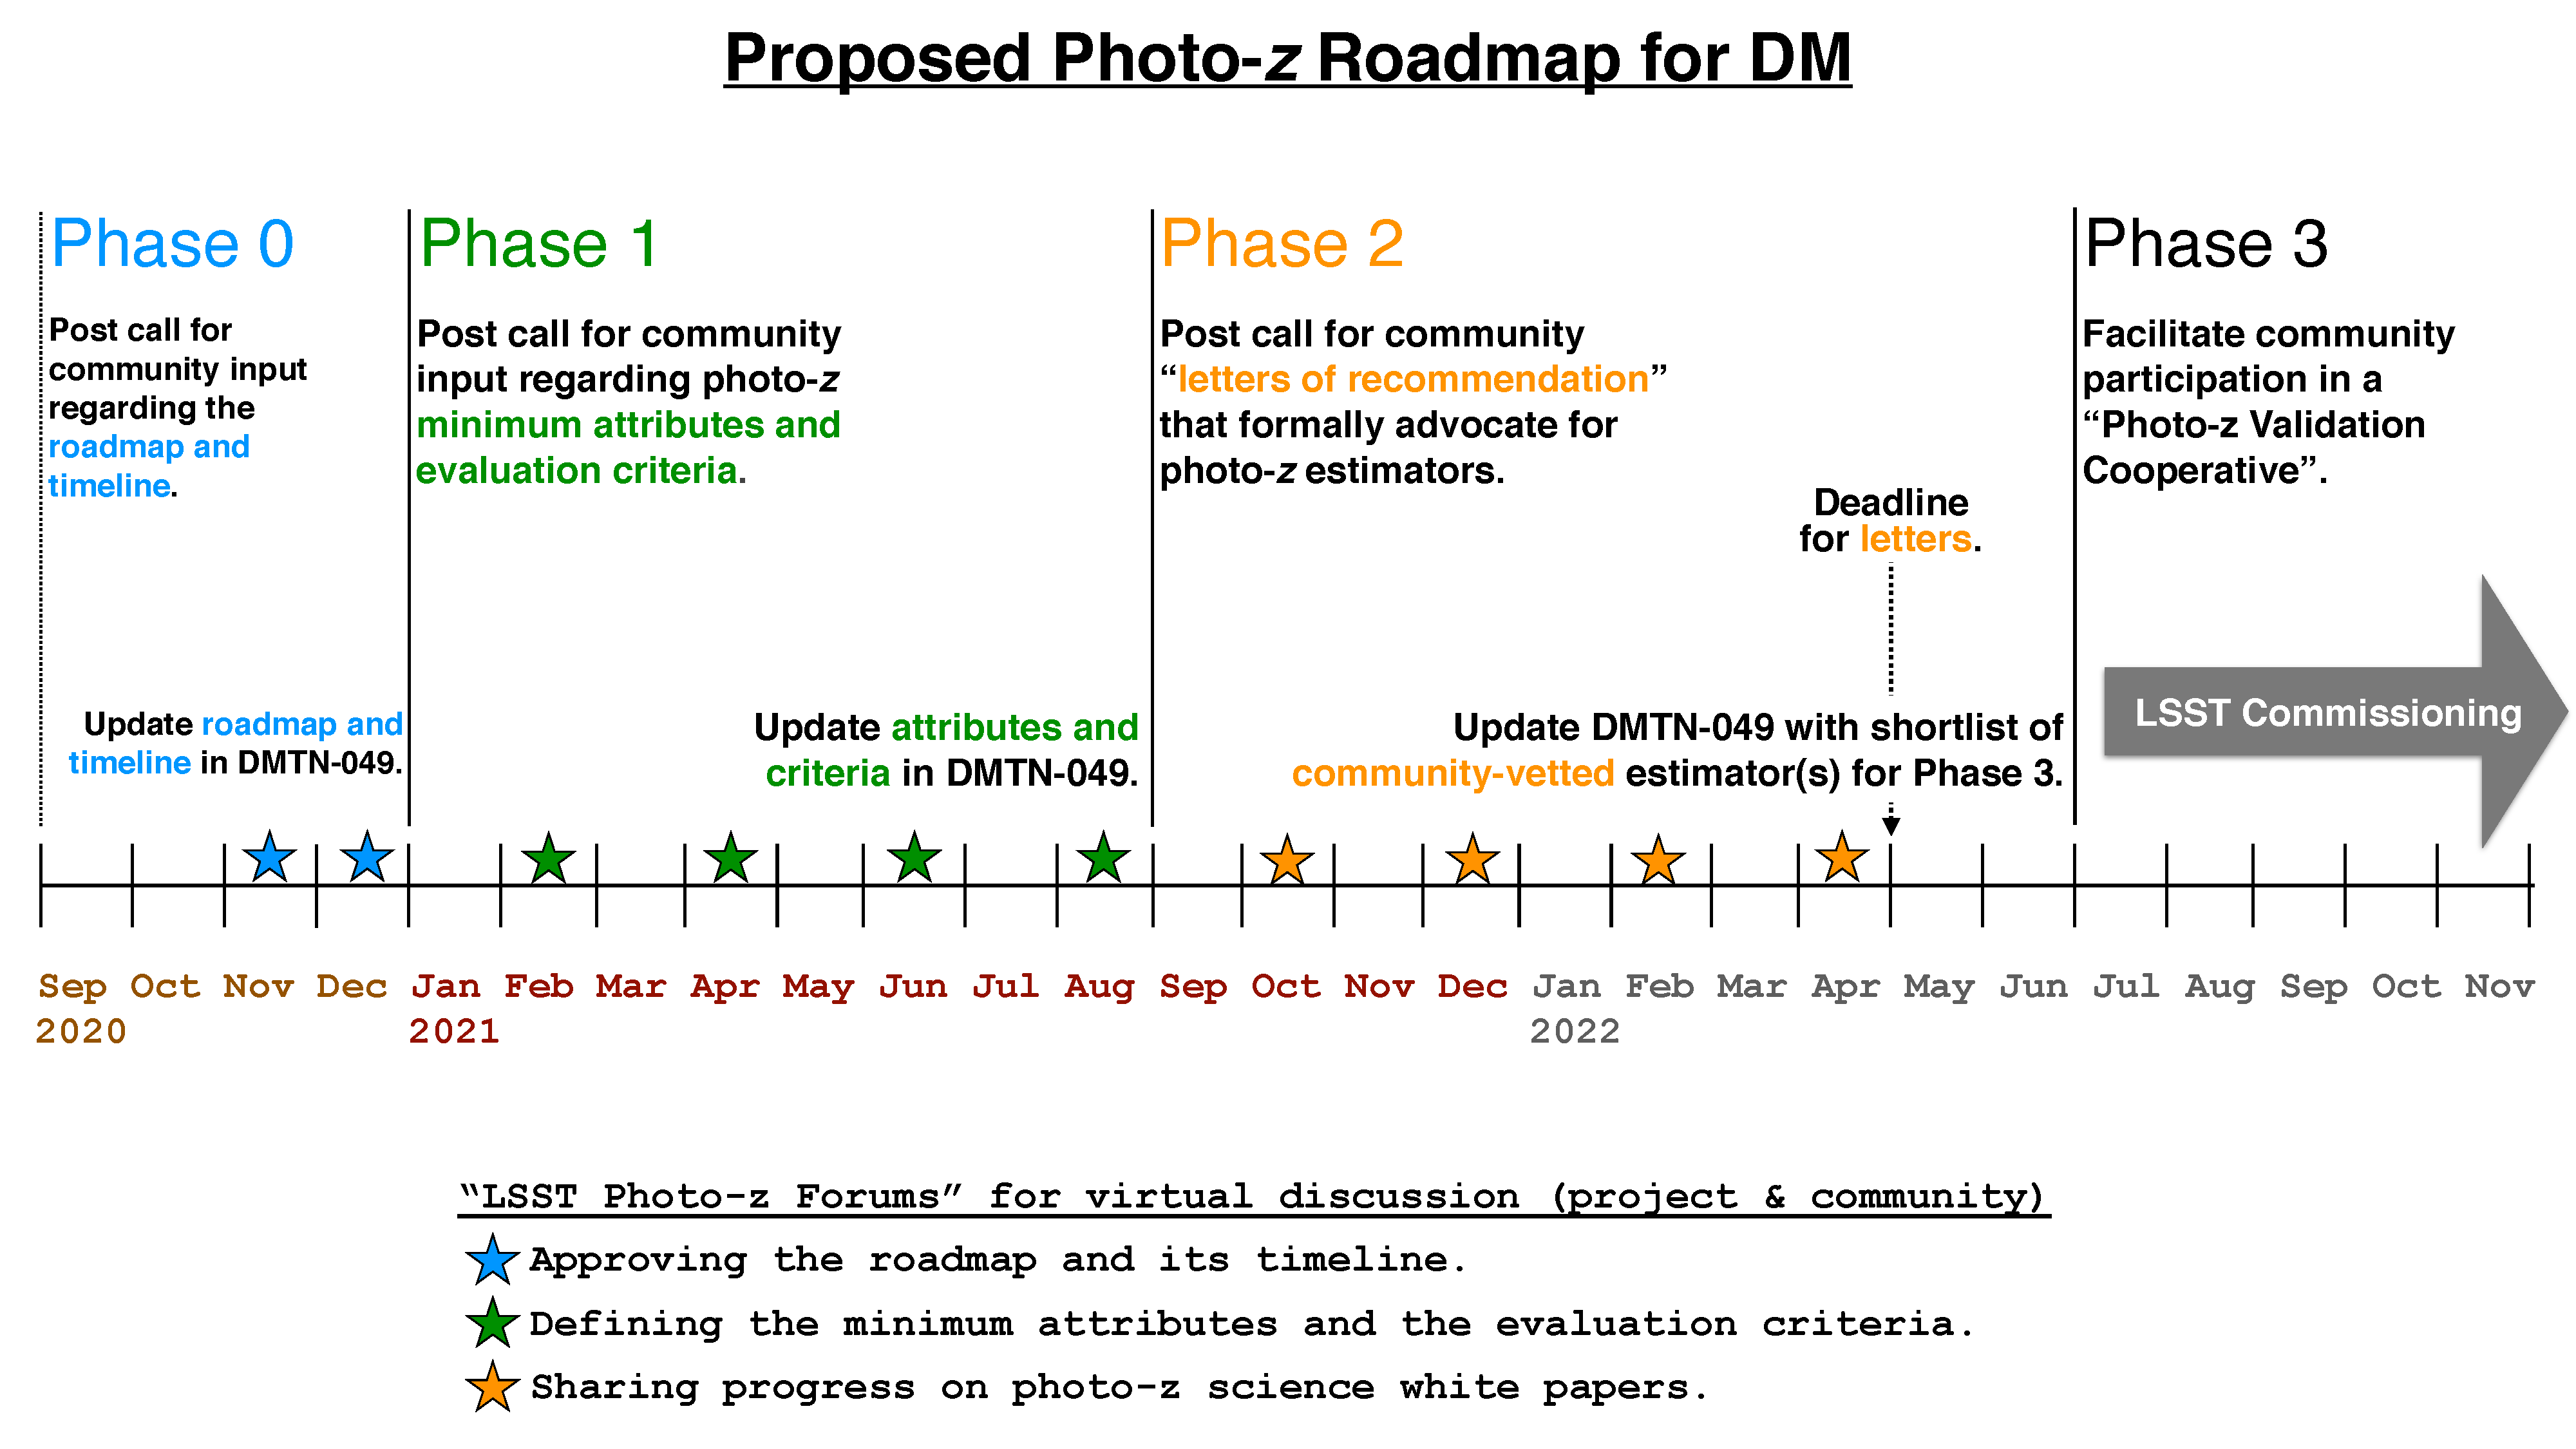
\includegraphics[width=17cm,trim=0cm 6cm 0cm 4cm, clip]{DMTN049_timeline.pdf}
\caption{A schematic of the proposed timeline of DM activities to engage the community in the roadmap to DR1 photo-$z$. In addition to the virtual forums (stars), community input will be ingested from asynchronus discussions in the Community Forum (Community.lsst.org). \label{fig:timeline}}
\end{center}
\end{figure}

\subsection{Phase 1: Define the Minimum Scientific Attributes and Evaluation Criteria}\label{ssec:time_mvp}

{\bf Jan 1 2021:} Write a solicitation for community input on the initial minimum scientific attributes (\S~\ref{sec:mvp}) and evaluation criteria (\S~\ref{sec:eval}) and advertise it broadly. \\
{\bf Feb -- Jun 2021:} Hold three LSST Photo-$z$ Virtual Forums that focus on gathering project and community input on the proposed minimum attributes and evaluation criteria. \\
{\bf mid-Aug 2021:} During the Rubin 2021 Project and Community workshop, hold a breakout session to collect any remaining input and discuss the evaluation criteria. \\
{\bf Aug 31 2021:} Incorporate community input into \S~\ref{sec:mvp} and \S~\ref{sec:eval} of this document.

\subsection{Phase 2: Prepare a Ranked List of Candidate Photo-$z$ Estimators}\label{ssec:time_wp}

{\bf Sep 1 2021:} Write a call for "Letters of Recommendation" from the science community that advocate for particular photo-$z$ estimators (\S~\ref{sec:lor}), and advertise it broadly. \\
{\bf Nov 2021 -- Apr 2022:} Hold four LSST Photo-$z$ Virtual Forums that focus on allowing the project and the community discuss the various merits or drawbacks photo-$z$ estimators. \\
{\bf Apr 31 2022:} Deadline for the science community's "Letters of Recommendation".\\
{\bf Jun 30 2022:} Generate a shortlist of community-vetted estimators to consider during Phase 3, and add the rationale for these choices to \S~\ref{ssec:lor_choice}.

\subsection{Phase 3: Facilitate the Photo-$z$ Validation Cooperative}\label{ssec:time_pzcoop}

{\bf During commissioning,} the DM team will facilitate community participation in a "Photo-$z$ Validation Cooperative", which will analyze photo-$z$ estimates from the shortlisted estimators based on commissioning data.
The timeline for this effort remains to be determined, as it is contingent on the commissioning schedule.
The DM team will make any final decisions regarding which photo-$z$ estimator(s) will be used for DR1 {\it after} this effort.
See \S~\ref{sec:pzcoop} for a preliminary description of the cooperative.


\subsection{Beyond DR1: Rubin Operations}\label{ssec:time_ops}

{\bf During operations,} the Data Production team will generate photo-$z$ for {\tt Object} catalogs using the software and data products delivered by the Construction-era DMS for DR1, and make available any and all supporting materials such as documentation or spectral templates.

The Rubin Operations team may solicit and collect community feedback on the photo-$z$ performance, and return to any stage of this roadmap to update the attributes, algorithms, implementation, and/or validation of {\tt Object} catalog photo-$z$ for future data releases.
Additionally (or instead of a DMS-provided photo-$z$), the Rubin Operations team might choose to federate a user-generated photo-$z$ catalog, as described below.

\subsubsection{Federation of a User-Generated Photo-$z$ Catalog}\label{ssec:time_ops_ugfed}

The Construction-era DMS delivered to the Operations Project will provide photo-$z$ with a basic level of scientific capability (\S~\ref{sec:mvp}). 
If those photo-$z$ are rendered obsolete by community efforts, and a superior user-generated photo-$z$ catalog is validated, {\it and} that catalog's creators are willing to share, then this data product should be ingested ("federated") and served with the {\tt Object} catalog.

As a long-term approach to providing DR {\tt Object} catalog photo-$z$, federating a user-generated catalog might require providing the community team(s) with access to data release previews (a small, e.g., $\sim10\%$, amount of a data release made available early, e.g., weeks to months, before the full release to enable community feedback and preparations prior to the full release).
This would enable the community team(s) to train and calibrate their photo-$z$ estimator, and would minimize the time between data release and federation of a new photo-$z$ catalog to the {\tt Objects} table (which is desired for many science goals, as described in Appendix \ref{ssec:use_none}).
Facilitating multiple teams sharing their photo-$z$ catalogs might involve hosting a "photo-$z$ server" within the Rubin Science Platform.
For example, the Dark Energy Survey's Science Portal is an infrastructure for organizing input catalogs, installing photo-$z$ estimators, training and running them, and evaluating their output\footnote{A series of YouTube tutorials about the DES Science Portal are available at \url{https://www.youtube.com/playlist?list=PLGFEWqwqBauBIYa8H6KnZ4d-5ytM59vG2}.}, as described by \citet{2018A&C....25...58G}).
Whether or not to federate user-generated photo-$z$ catalogs remains a decision for the Operations team.

\subsection{International Partnerships (In-Kind Contributions)}\label{ssec:time_inkind}

{\bf At all stages of this photo-$z$ roadmap,} in-kind program contributions related to photo-$z$ should be included and integrated into the communal efforts to optimize the LSST photo-$z$. 
These contributions might include, e.g., individuals' expertise; scientific analyses; software algorithms, tools, or infrastructure; computational resources; datasets or observing time.
These contributions might be directed to the Project (e.g., DM, commissioning team), and/or to the science community (e.g., a Science Collaboration, all data rights holders). 

In-kind teams should expect to work closely with the project (e.g., DM) and other Rubin community members on each step of this proposed roadmap, including the solicitation of input from the science community, the process of implementation and validation, and maintaining and evolving their contributions during Rubin Operations (as applicable).
In-kind contributors should also review the summary of related data products and documentation that might pertain to their contribution (Appendice \ref{sec:dp} and  \ref{sec:docs}), and the example scientific use-cases that the photo-$z$ estimates are expected to support (Appendix \ref{sec:use}).

For in-kind programs making photo-$z$ related contributions to the project, a Photo-$z$ In-Kind Program Coordination (IPC) group exists to facilitate communications (point of contact: Melissa Graham). See this post in the Community Forum for more information: \url{https://community.lsst.org/t/about-the-photo-z-in-kind-coordination-group}.



\clearpage
% % % % % % % % % % % % % % % % % % % % % % % % % % % % % %
\section{Data Management Constraints on the Photo-$z$ Estimator(s)}\label{sec:dmcon}

\textit{This is where DM must write down the constraints on the photo-$z$ estimators, in order to provide the community with some boundaries and expectations. Compliance with these constraints is one of the proposed evaluation criteria in \S~\ref{sec:eval}.}

\textbf{Supported Languages: } \textit{Does the code have to be in, e.g., C or Python?}

\textbf{Storage Constraints: } \textit{Maximum storage space for: inputs such as spectral templates or training sets (Appendix \ref{ssec:dp_calib}); inputs such as photometric measurements, and they must already exist in the {\tt Object} catalog (Appendix \ref{ssec:dp_objvals}); outputs such as posteriors (Appendix \ref{ssec:dp_pz}).}

\textbf{Computational Processing Constraints: } \textit{What is the maximum processing load? If outputs are going to be compressed (Appendix \ref{ssec:dp_store}), what are the constraints on doing this compression?}

\textbf{Other: } \textit{?}




\clearpage
% % % % % % % % % % % % % % % % % % % % % % % % % % % % % %
\section{Proposed Initial Minimum Scientific Attributes (Phase 1)}\label{sec:mvp}

The following is a \textbf{\textit{preliminary draft}} set of {\it proposed initial} minimum scientific attributes for {\tt Object} catalog photo-$z$.
\textbf{Community input on these proposed minimum scientific attributes is solicited during Phase 1}, as is input on the supporting material that motivates these attributes (Appendices \ref{sec:dp} and \ref{sec:use}).
The following will be updated to reflect community input prior to Phase 2.

The minimum scientific attributes should be based on the guiding principle that the DMS-generated {\tt Object} photo-$z$ should, at minimum, {\it meet the basic science needs for communities which will not or cannot generate custom photo-$z$} and also DM's internal use-cases (Appendix \ref{sec:use}).
A {\it basic} science need would not include, for example, photo-$z$ of the quality required for major cosmological advances.
The development of such photo-$z$ algorithms is an active research topic within the Dark Energy Science Collaboration \citep{2018arXiv180901669T}, and a significant effort which the Rubin Observatory staff should not (and could not) attempt to replicate. 

{\bf Draft: Type of Estimator --} 
The {\tt Object} catalog photo-$z$ estimates should be based on a template-fitting algorithm {\it and then also} a machine-learning algorithm, if multiple results can be stored (see Appendix \ref{ssec:dp_store}).
The main motivation for this is galaxies-related science (Appendix \ref{sssec:use_sci_gal}) and internal (Appendix \ref{ssec:use_dm}) use-cases, which would use the best-fit template to derive additional galaxy properties.

{\bf Draft: Output Format --} 
The {\tt Object} catalog photo-$z$ should include the posterior distribution function and a point estimate with an uncertainty, as well as reliable uncertainties and/or flags to help the novice user avoid misinterpreting the results or overestimating their significance.
For template-fit photo-$z$ results, an identifier for the best-fit template should be provided, and those templates be made publicly accessible.
A list of the photo-$z$ outputs (and associated documentation) is put forth in Appendix \ref{ssec:dp_pz}.

{\bf Draft: Performance --} 
Based on the science use-cases in Appendix \ref{sec:use}, the {\tt Object} catalog photo-$z$ could have a point-estimate accuracy of $\sim10\%$ and still meet the basic science needs.
The photo-$z$ results should result in a standard deviation of $z_{\rm true}-z_{\rm phot}$ of $\sigma_z < 0.05(1+z_{\rm phot})$, and a catastrophic outlier fraction of $f_{\rm outlier} < 10\%$, over a redshift range of $0.0 < z_{\rm phot} < 2.0$ for galaxies with $i<25$ mag galaxies.


\clearpage
% % % % % % % % % % % % % % % % % % % % % % % % % % % % % %
\section{Proposed Evaluation Criteria (Phase 1)} \label{sec:eval}

The following is a \textbf{\textit{preliminary draft}} set of proposed evaluation criteria for photo-$z$ estimators. 
\textbf{Community input on these proposed evaluation criteria is solicited during Phase 1}, as is input on the supporting material that motivates these attributes (Appendices \ref{sec:imp}, \ref{sec:dp}, and \ref{sec:use}).
The following will be updated to reflect community input prior to Phase 2.

These evaluation criteria are needed to guide the contents of the community's "Letters of Recommendation" in Phase 2 (\S~\ref{sec:lor}).
These criteria would also apply to any user-generated catalogs to be federated with the {\tt Objects} table (Appendix \ref{ssec:time_ops_ugfed}).

{\bf Draft: Meeting the Defined Minimum Attributes --}
Estimators should meet the minimum attributes defined in \S~\ref{sec:mvp}, and meet the basic science needs of the community and any internal DM use-cases (Appendix \ref{sec:use}).
Note that the preliminary proposed performance (\S~\ref{sec:mvp}) has been shown to be achievable for simulated LSST data with existing photo-$z$ estimators \citep[e.g.,][]{2018AJ....155....1G,2020arXiv200103621S}.

{\bf Draft: Scientific Utility and User Experience --}
Photo-$z$ estimators should serve as wide a variety of science needs as possible (Appendix \ref{sec:use}), and should enable early science in particular (Appendix \ref{ssec:use_LOY1}).
It is beneficial if estimators have demonstrated success with other wide-field optical surveys, especially for surveys that overlap with LSST (for results comparisons), and have broad community adoption.
The estimators' data products should be straightforward to understand and easy to access (described further in Appendix \ref{ssec:dp_pz}).
Estimators should have publicly accessible documentation (e.g., journal article, website, schema) to facilitate community use.

{\bf Draft: Implementation, Validation, and Computational Requirements --}
The computational processing and storage needs of the estimator must fit within the available resources of the data facility, and it must be able to run within the DR pipelines, meeting all constraints defined in \S~\ref{sec:dmcon}. 
New algorithmic development is beyond the scope of DM, and the estimators should not need any expansion or maturation prior to installation in the DMS.
Estimators should take as inputs quantities that the LSST pipelines are planning to produce (Appendix \ref{ssec:dp_objvals}).
The implementation process should be straightforward (Appendix \ref{sec:imp}).
The necessary data -- from LSST or elsewhere -- for training, calibration, and validation must exist during the Rubin Observatory commissioning phase and be available for the "Photo-$z$ Validation Cooperative" (Appendix \ref{ssec:dp_calib}).
%\textcolor{red}{The process of implementation and validation should require no more personnel hours than are available for the task.}



\clearpage
% % % % % % % % % % % % % % % % % % % % % % % % % % % % % %
\section{Community "Letters of Recommendation" (Phase 2)} \label{sec:lor}

\textbf{This preliminary draft call for letters of recommendation will be updated based on community input ingested during Phase 1.}

\textbf{Draft:} \\
It is recognized that the Rubin community has a considerable depth of expertise regarding photometric redshifts and the potential scientific impacts of the choice of estimator(s) to use for DR1.
This phase focused on letters of recommendation are a formal chance for the science community to state their scientific needs regarding {\tt Object} catalog photo-$z$.

The goal is to create a shortlist of several community-vetted photo-$z$ estimator(s) that will serve as broad a range of LSST science goals as possible and also meet internal (DM use-case) requirements.
This shortlist would then serve to coalesce the joint efforts of DM and the community during the  "Photo-$z$ Validation Cooperative", which will be based on commissioning data (\S~\ref{sec:pzcoop}). 

Based on the above goals, these "letters of recommendation":
\begin{itemize}
\item should focus on the science-driven prioritization of photo-$z$ estimators that is informed by the evaluation criteria in  \S~\ref{sec:eval}
\item should be short (i.e., 1 page, ideally), and should not constitute an onerous task
\item could focus on many, a few, or just one estimator(s) or science goal(s)
\item could be primarily {\it qualitative} in their evaluation of the photo-$z$ estimators
\item could include {\it quantitative} analyses of simulated LSST data, or data from other facilities (but more likely would just cite such quantitative analyses)
\item will be openly shared in the Rubin community
\end{itemize}


\subsection{Shortlisted Photo-$z$ Estimator(s)} \label{ssec:lor_choice}

\textit{TBD: This section will summarize the Letters of Recommendation and describe which community-vetted photo-$z$ estimator(s) have been shortlisted for the photo-$z$ validation cooperative, and why.}


\clearpage
% % % % % % % % % % % % % % % % % % % % % % % % % % % % % %
\section{Photo-$z$ Validation Cooperative (Phase 3)}\label{sec:pzcoop}

\textbf{This preliminary draft description of this proposed cooperative effort will be updated based on community input, which is welcome at any time.}

\textbf{Draft:} \\
As the scientific community has a considerable wealth of expertise in generating photo-z catalogs, and will be the primary users of the photo-z data product, they are the best suited to scientifically validate the {\tt Object} catalog photo-$z$.
Towards this end the DM team plans to facilitate a "Photo-$z$ Validation Cooperative" to analyze photo-$z$ estimates based on LSST commissioning data and share results.
This is intended to be a collaborative endeavor between project and community to maximize the scientific utility of the {\tt Object} catalog photo-$z$ data products.

It is anticipated that this process will start with open communication about what the science community needs to fully participate in the photo-$z$ co-op (e.g., commissioning data, access to tools, computational resources).
During this process, DM will focus on providing technical support for the validation of the photo-$z$ estimators using commissioning data, especially those shortlisted based on the community's letters of recommendation (\S~\ref{sec:lor}), but the community may also consider estimator(s) that were not shortlisted.
It is expected that the community will be focused on assembling training sets and validation metrics and applying them to the commissioning data, and documenting and sharing the results.
The mode of communication during this time (e.g., an extension of the "Photo-$z$ Virtual Forums") remains to be determined.

Types of commissioning data that might be most useful for scientific validation of photo-$z$ estimators are described in \S~\ref{ssec:pzcoop_commissioning}.
A preliminary collection of photo-$z$ validation techniques based are presented in Appendix \ref{sec:imp}, and a preliminary collection of training and calibration data in Appendix \ref{sec:dp}.

Documentation regarding the technical aspects of the implementation and validation process is considered beyond the scope of this document and will appear elsewhere.

\subsection{Potential Commissioning Data for Photo-$z$ Validation}\label{ssec:pzcoop_commissioning}

The commissioning surveys and their schedule remained subject to change; the examples below will be updated in the future as the situation clarifies.

{\bf Data Preview 1 (DP1):} The first phase of commissioning with ComCam might include, e.g., tests of the scheduler; tests of image quality, depth, astrometry, and photometry; and a 20-year depth test to stack images over a range of conditions \citedsp{LSE-79}.
DP1 might be useful as preliminary test data during the implementation of the photo-$z$ estimators, and help to test the formats of the input and output data, create visualizations for the validation codes, etc.

{\bf Data Preview 2 (DP2):} The second phase of commissioning with the Science Camera might include, e.g., wide area surveys to the full 10-year depth in addition to a 20-year depth stack and tests of image quality, as in DP1 \citedsp{LSE-79}.
DP2 is more likely to provide the data set for photo-$z$ validation, and also some of the needed training data for LSST photo-$z$ described in Appendix \ref{ssec:dp_calib}.
Covering well-studied fields during DP2 (e.g., COSMOS) would facilitate photo-$z$ validation; note that the effort to collect community input on the commissioning fields is underway\footnote{\url{https://community.lsst.org/t/community-input-to-the-on-sky-observing-strategy-during-commissioning}}.

As a side note for LSST users who are interested in doing science with commissioning data: it should not be assumed that any release of data products based on commissioning surveys will include photo-$z$ estimates.
The release of any photo-$z$ catalogs prior to DR1 remains at the discretion of the DM team.




\clearpage
% % % % % % % % % % % % % % % % % % % % % % % % % % % % % %
\bibliography{lsst,refs_ads,local}

\clearpage
% % % % % % % % % % % % % % % % % % % % % % % % % % % % % %
\appendix 

%% % % % % % % % % % % % % %
%\subsection{Mario's Original Roadmap to Photo-$z$}\label{ssec:dmcalc_mario}
%This option has served as the basis for our discussions with the science community since 2016, and is based on comments by Mario Juri\'{c} on the Jira thread DM-6367.
%The process for the definition of the Data Release (DR) photo-$z$ data product is:
%\begin{enumerate}[noitemsep,topsep=-10pt]
%\item DM Project Science (acting on behalf of overall Project Science) consults with the community (represented by the relevant collaboration -- in this case, the DESC) for proposed options regarding the most appropriate algorithm and format for the results. Iteration between DM and the science community will be necessary in order to converge to a scientifically acceptable {\it and} implementable solution (e.g., if DESC recommends an algorithm that does not meet DM's computational, storage, or budget limitations, or if DESC recommends an algorithm that the other SC have concerns with).
%\item Following that (iterative) consultation, DM will recommend (and the Project will select) the photo-$z$ algorithm and the data product format to be incorporated into DR Processing.
%\item DM will implement the selected algorithm, using whatever they can transfer over from DESC (or other) work, but DM's requirements may be higher than DESC's (e.g., the algorithm will need to run reliably in LSST's production environment).
%\item DM will implement anything needed to integrate, verify, validate, and run QA on the photo-$z$ data product in data releases (and everything leading up to the annual releases; e.g., commissioning), because photo-$z$ are ultimately a Project deliverable.
%\end{enumerate}

\clearpage
% % % % % % % % % % % % % % % % % % % % % % % % % % % % % %
\section{Appendix: Examples of Implementation and Validation}\label{sec:imp}

\subsection{An Example Implementation Process}\label{ssec:imp_imp}

For reference, the basic steps for implementing a photo-$z$ estimator include:
\vspace{-15pt}
\begin{itemize}
\item prepare the LSST data inputs to the photo-$z$ estimators (Appendix \ref{ssec:dp_objvals})
\item prepare the training and calibration data (Appendix \ref{ssec:dp_calib})
\item install the needed codes (a technical aspect to be described elsewhere)
\item run the estimator (on its own and/or embedded in the data release pipeline)
\item validate the photo-$z$ estimator outputs (below, \ref{ssec:imp_val})
\item store the results in the {\tt Object} catalog (Appendices \ref{ssec:dp_pz} and \ref{ssec:dp_store})
\item ensure output schema and access methods are documented (Appendix \ref{ssec:dp_pz})
\end{itemize}

\subsection{Example Validation Tests}\label{ssec:imp_val}

For reference, this section describes some photo-$z$ validation tests, some of which overlap with the evaluation criteria described in \S~\ref{sec:eval}. 
Validation tests and quality assessment diagnostics will be necessary to ensure the results meet performance expectations (\S~\ref{sec:mvp}).
These lists are based in part on a brainstorming session during the LSST Project and Community Workshop's session on Photometric Redshifts on Aug 14 2019\footnote{E.g., slide 14 of \url{https://docs.google.com/presentation/d/1GEahvDQXIjSL4lLVjDlZHV5zpXLhGQfHwVtucs72Ajg/edit?usp=sharing}}.

Journal articles that demonstrate validation processes for photo-$z$ from multi-band wide-area surveys include {\it "DES science portal: Computing photometric redshifts"} \citep{2018A&C....25...58G}; {\it "Photometric redshifts for Hyper Suprime-Cam Subaru Strategic Program Data Release 1"} \citep{2018PASJ...70S...9T}; and {\it "On the realistic validation of photometric redshifts"} \citep{2017MNRAS.468.4323B}. 

{\bf Truth Comparisons --} 
Catalogs of true redshifts can be obtained by withholding some fraction of the training set or by cross-matching to external spectroscopic catalogs. Validation metrics should include at least those used to define the minimum performance of the LSST photo-$z$ for basic science needs (\S~\ref{sec:mvp}). A list of potential metrics might include the following, and targets or limits on these metric values might apply to subsets in magnitude, color, or redshift: 
\vspace{-15pt}
\begin{itemize}
\item plots of $z_{\rm true}$ {\it vs.} $z_{\rm phot}$ for visual inspection
\item standard deviation and bias in $\Delta z = (z_{\rm true}-z_{\rm phot})/(1+z_{\rm true})$
\item fraction of (catastrophic) outliers, e.g., $\Delta z > 3\sigma$ or $>0.06$ ($>1$)
\item quantile-quantile (q-q) plots evaluate the shape of $P(z)$
\item probability integrated transform, $PIT(z_{\rm phot}) = \int_{0}^{z_{\rm phot}} P(z)\,dz$, calculated for all test galaxies, should be flat for well-estimated $P(z)$ \citep{2016arXiv160808016P}
\item the continuous ranking probability score, CRPS, should be a lower value for better estimated $P(z)$, as described in \citep{2016arXiv160808016P}
\item redshift confidence for point estimates, $C(z_{\rm phot}) = \int_{z_{\rm phot}-0.03}^{z_{\rm phot}+0.03} P(z)\,dz $
\item loss and risk parameters that characterize the photo-$z$ estimates:\\
$L(\Delta z) = 1 - \left(1+ \left(\frac{\Delta z}{\gamma} \right)^2 \right)^{-1}$, 
where $\gamma$ is a characteristic threshold (e.g., $0.15$), and:\\
$R(z_{\rm phot}) = \int P(z)\,L(z_{\rm phot},z)\,dz$, as described in \citet{2018PASJ...70S...9T}
\item the conditional density estimation (CDE) loss as described in Section 4.2 of \citet{2020arXiv200103621S}. (Note that the CDE does not strictly require the true posterior be known.)
\end{itemize}

{\bf Sanity Checks--} 
These are tests that can be done using all LSST {\tt Objects} and do not require a truth catalog.
\vspace{-15pt}
\begin{itemize}
\item the uncertainty in $z_{\rm phot}$ should correlate with photometric error
\item the star/galaxy flag parameter should agree with photo-$z$ (stars have $z_{\rm phot}=0$)
\item evolution of $N(z)$ to higher-$z$ for samples with fainter magnitudes, redder colors
\end{itemize}

{\bf Scientific Applications --} 
The following might not be included in the formal validation process, but represent analyses that the broader scientific community may want to do to inform their use of the LSST photo-$z$.
\vspace{-15pt}
\begin{itemize}
\item assessing the performance of point estimates in broker photometric classification algorithms
\item evaluating the absolute magnitude distribution of Type Ia supernovae once the distance derived from the photo-$z$ point estimates are applied
\item evaluating the distributions of derived physical parameters for galaxies using the $P(z)$
\item checking whether high SFR galaxies (and maybe other sensitive populations) have reasonable $P(z)$
\item galaxy cluster membership identification
\item tomographic bin analysis, as in \citep{2019MNRAS.482.2807C}
\end{itemize}


\subsection{Example Publications that Evaluate Photo-$z$ Estimator Performance}\label{ssec:imp_evalpubs}

\begin{itemize}
\item \citet{2010A&A...523A..31H} tested 18 different photo-$z$ codes on the same sets of simulated and real data and found no significantly outstanding method.
\item \citet{2013ApJ...775...93D} tested 11 different photo-$z$ codes on the CANDLES data set ($U$-band through infrared photometry) and also find that no method stands out as the "best'', and that most of the photo-$z$ codes underestimate their redshift errors.
\item \citet{2014MNRAS.445.1482S} used the science verification data (200 square degrees of $grizY$ photometry to a depth of $i_{AB}=24$ magnitudes) of the Dark Energy Survey (DES) to evaluate several photometric redshift estimators. They found that the Trees for Photo-$z$ code (TPZ; \citet{2013ascl.soft04011C}) provided the most accurate results with the highest redshift resolution, and that template-fitting methods also performed well -- especially with priors -- but that in general there was no clear "winner.''
\item \citet{2018PASJ...70S...9T} provides a comparative analysis of several photo-$z$ estimators applied to their data set from the HSC Strategic Program. Their website\footnote{\url{https://hsc-release.mtk.nao.ac.jp/doc/index.php/photometric-redshifts/}} provides comparative analysis plots for each of them.
\item \citet{2020arXiv200103621S} statistically compare the posterior probability distribution functions produced by 12 photo-$z$ estimators for a mock data set that is representative of the LSST, identifying some biases and shortfalls in both the produced PDFs and the evaluation methods used to analyze them.
\end{itemize}



\clearpage
% % % % % % % % % % % % % % % % % % % % % % % % % % % % % %
\section{Appendix: Data Products Related to LSST Photo-$z$}\label{sec:dp}

For reference, this section provides a \textbf{\textit{preliminary and incomplete}} collection of inputs, outputs, and associated products related to generating and serving LSST photo-$z$:
\begin{itemize}
\item the LSST data products needed as input to photo-$z$ estimators (Appendix \ref{ssec:dp_objvals})
\item the required training and calibration data, LSST or external (Appendix \ref{ssec:dp_calib})
\item the outputs' format, access methods, and documentation (Appendix \ref{ssec:dp_pz})
\item options for compression to store the results of multiple estimators (Appendix \ref{ssec:dp_store})
\end{itemize}


\subsection{Inputs to Photo-$z$ Estimators}\label{ssec:dp_objvals}

It is important to ensure that all measured quantities needed by photometric redshift estimators are going to be computed and included in the {\tt Object} table. 
Aside from the fluxes and/or apparent magnitudes and errors for each Rubin Observatory filter, which will be provided in the {\tt Object} catalog, the color properties in the {\tt Object} table might be used for photo-$z$. {\it "Colors of the object in 'standard seeing' (for example, the third quartile expected survey seeing in the i band, $\sim$0.9 arcsec) will be measured. These colors are guaranteed to be seeing-insensitive, suitable for estimation of photometric redshifts"} \citedsp{LSE-163}. In the {\tt Object} table the relevant elements are:
\vspace{-15pt}
\begin{itemize}
\item \texttt{stdColor (float[5])} = {\it 'standard color', color of the object measured in 'standard seeing', suitable for photo-$z$}
\item \texttt{stdColorErr (float[5])} = {\it uncertainty on \texttt{stdColor}}
\end{itemize}

Additionally, measured quantities such as the galaxy size, shape, radial profile, 'clumpiness', or surface brightness; the DCR correction (or residual); or a parameter that represents the clustering density within some radius (e.g., 2 Mpc) might all be useful (e.g., as priors) for photo-$z$ estimators. The effective transmission function ($\phi$; Eq. 5 in \citeds{LPM-17}), which will be provided for all {\tt Sources} either in the catalog or as a link, is another useful quantity for photo-$z$ estimators.


\subsection{Training and Calibration Data}\label{ssec:dp_calib}

{\bf Spectroscopic Redshifts --}
Deep multi-band LSST photometry for spectroscopic fields like COSMOS, and/or WFD-depth LSST photometry that overlaps multiplexed spectroscopic surveys like DESI/4MOST, which is obtained either during commissioning or early in Operations year 1, will likely be necessary to produce photo-$z$ for DR1.

{\bf Wide Area Imaging --} 
Some photo-$z$ methods have requirements other than spec-$z$ fields: e.g., \citet{2019MNRAS.483.2801S} use clustering information to obtain photo-$z$ and this requires wider, shallower field coverage and not a single deep pointing like a spec-$z$ field would have. 
This wider area would also serve to reduce cosmic variance in the training set ($\sim$100 square degrees would serve to average out the variance).

{\bf Data Previews --}
For the community to participate in the training or calibration of a photo-$z$ estimator prior to a data release, it will probably be necessary to release a small ($\sim10\%$) but representative "DR preview" in advance of each data release during Operations.


\subsection{Output Schema, Access Methods, and Documentation}\label{ssec:dp_pz}

{\bf Output Schema --} 
The format of the photo-$z$ output is one of the minimum attributes that must still be defined (\S~\ref{sec:mvp}). 
The photo-$z$ outputs must provide all the necessary inputs to the validation tests, to be defined in Appendix \ref{ssec:imp_val}.
The currently proposed {\tt Object} catalog table elements related to photo-$z$ are defined in \citeds{LSE-163} and provided in \S~\ref{ssec:docs_dpdd}, and summarized here:
\vspace{-15pt}
\begin{itemize}
\item posterior probability distribution function (likelihood over redshift)
\item a single point estimate with an uncertainty
\item quantities related to the posterior (e.g., mode, mean, skewnewss)
\item flags (e.g., potential catastrophic outlier, failure mode, consistent with z=0)
\end{itemize}

{\bf Access Methods --} 
The user experience is one of the proposed selection criteria for the LSST photo-$z$ estimator (\S~\ref{sec:eval}). 
Some examples of publicly released photo-$z$ catalogs which were prepared with a user experience that might be desirable for the LSST photo-$z$ include the Dark Energy Survey's Science Portal to serve photometric redshifts \cite{2018A&C....25...58G} and the Hyper SuprimeCam Subaru Strategic Program \cite{2018PASJ...70S...9T}\footnote{\url{https://hsc-release.mtk.nao.ac.jp/doc/index.php/photometric-redshifts/}}.

If the LSST photo-$z$ are not made available in either the {\tt Objects} table or in a federated or joinable catalog -- for example in the case where a community-generated photo-$z$ catalog is replacing the DMS-generated catalog (Appendix \ref{ssec:time_ops_ugfed}) -- and are instead made available via, e.g., a "photo-$z$ server" (as in \cite{2018A&C....25...58G}), then at least the {\tt Object} catalog ID of the most recent data release should be a queryable parameter.

If the results of multiple estimators are generated, compressed, and stored in the {\tt Objects} table, then decompression should be straightforward for the user (Appendix \ref{ssec:dp_store}).

{\bf Documentation --} 
Appropriate types of documentation might include published journal articles, GitHub repositories, websites, or other online documentation resources (e.g., \url{https://readthedocs.org/}). Whatever the format, the documentation contents should include: 
\vspace{-15pt}
\begin{itemize}
\item general description of the estimator
\item adaptations made to ingest LSST data (compared to past applications)
\item an analysis of the training, calibration, and validation processes
\item a full list of all inputs and outputs (i.e., a schema browser)
\end{itemize}

\subsection{Storage and Compression}\label{ssec:dp_store}

The stored values related to photo-$z$ are subject to the storage space allotted in the {\tt Objects} table as described in \S~\ref{ssec:docs_dpdd}.
Both the posteriors and point estimates from several different photo-$z$ estimators could be compressed and stored in this allotted space.
Given the variety of use-cases and the fact that different photo-z estimators produce different results \citep{2020arXiv200103621S}, the option to compute, compress, and store estimates from multiple estimators in the $2\times95$ float might be scientifically desirable.

Efficient $P(z)$ compression algorithms are in development, such as \citet{2014MNRAS.441.3550C} and \citet{2018AJ....156...35M}.
\citet{2014MNRAS.441.3550C} present an algorithm for sparse representation, for which {\it "an entire PDF can be stored by using a 4-byte integer per basis function''} and {\it "only ten to twenty points per galaxy are sufficient to reconstruct both the individual PDFs and the ensemble redshift distribution, $N(z)$, to an accuracy of 99.9\% when compared to the one built using the original PDFs computed with a resolution of $\delta z = 0.01$, reducing the required storage of two hundred original values by a factor of ten to twenty.''} 
\citet{2018AJ....156...35M} presents a {\tt Python} package for compressing one-dimensional posterior distribution functions (PDFs), demonstrates its performance on several types of photo-$z$ PDFs, and provides a set of recommendations for best practices which should be consulted when DM is making decisions on the DR photo-$z$ data products.

However, compression (and decompression by users) will require extra computational resources, which should be estimated and considered, and decompression must be fast and easy for users.


\clearpage
% % % % % % % % % % % % % % % % % % % % % % % % % % % % % %
\section{Appendix: Example Use-Cases for LSST Photo-$z$} \label{sec:use}

This section contains an \textbf{\textit{incomplete, non-exhaustive}} summary of a variety of internal and scientific use-cases for the LSST {\tt Object} catalog photo-$z$.
These use-cases inform the minimum attributes and selection criteria proposed in \S~\ref{sec:mvp} and \ref{sec:eval}. 

Some of the following information on use-cases was collected from participants of the LSST Project and Community Workshop's session on Photometric Redshifts on Aug 14 2019\footnote{Thanks to Sam Schmidt, Chris Morrison, Sugata Kaviraj, Gautham Narayan, Lauren Corlies, Travis Rector, Tina Peters, Alex Malz, Dara Norman, Stephen Smartt, and other participants from the science community.}.

\subsection{Internal DMS Use-Cases}\label{ssec:use_dm}

DM's galaxy photometry outputs are being developed with the goal of feeding photometric redshift estimators, so the computation of photometric redshifts is likely to be a part of the science validation process for LSST photometry. 
Unlike stars, color-color and color-magnitude diagrams for galaxies do not have sufficient structure to reveal issues with the photometry.
While other photometric validation techniques will also be useful (such as evaluating the width of galaxy cluster red-sequences) they may only apply to {\it some} galaxies, whereas {\it all} galaxies have a redshift. 

The internal use-case of scientifically validating the galaxy photometry outputs is likely to require a simple photo-$z$ estimator which fits SED templates, since the goal is to evaluate whether the photometric outputs match the colors of real galaxies.
Whether such a simple SED-fit photo-$z$ could also serve the scientific use-cases is undetermined, because the photometric validation process is not yet defined or written.
The internal use-case described in \S~\ref{ssec:docs_oss} -- of needing photo-$z$ in order to assess catalog completeness for low- and high-redshift {\tt Objects} -- is also likely to be served by a simple SED-fit photo-$z$ estimate.

As a side note, although the DMS will assign fiducial spectral energy distributions (SEDs) to {\tt Objects} in order to apply sub-band wavelength-dependent photometric calibration and PSF modeling, computing photo-$z$ is not planned to be a part of this process.
Furthermore, the SED templates used will likely be simpler (e.g., step-function or slope) than would be needed for deriving photo-$z$.

\subsection{Scientific Use-Cases}\label{ssec:use_sci}

A variety of potential scientific applications for the {\tt Object} photo-$z$ are discussed in turn. 
These scientific use-cases should be used to inform the minimum attributes and selection criteria proposed in \S~\ref{sec:mvp} and \ref{sec:eval}.
A summary of the commonalities between science use-cases for photo-$z$ is provided in \S~\ref{sssec:use_sci_sum}.

\subsubsection{Dark Energy}\label{sssec:use_sci_de}
Extragalactic astrophysics such as weak lensing, baryon acoustic oscillations, and Type Ia supernova cosmology are all main science drivers for the LSST, and all require catalogs of galaxies with photometric redshifts.
The photo-$z$ estimators for precision cosmology will be custom-tailored to these particular science goals, and the photo-$z$ results are subject to established science requirements for dark energy cosmology \citep{2018arXiv180901669T}.
For example, weak lensing and large scale structure require ensemble measurements of $N(z)$ and thus require a full posterior PDF, whereas point-estimate photo-$z$ for individual {\tt Objects} are required for Type Ia supernova host galaxies and the identification of strong lensing candidates and galaxy cluster members. 
The Dark Energy Science Collaboration (DESC) is developing specialized photo-$z$ pipelines for these science goals (which {\it could} serve to generate photo-$z$ for the {\tt Object} catalog, as discussed in Appendix \ref{ssec:time_ops_ugfed}).

\subsubsection{Time Domain}\label{sssec:use_sci_td}
The Transients and Variable Stars Science Collaboration reported that they would use LSST-provided {\tt Object} photo-$z$ to identify and/or characterize extragalactic transient host galaxies.
Alert packets provide {\tt Object} IDs for the three nearest stars and three nearest galaxies in the most recent data release.
Alert stream brokers intend to query the {\tt Objects} catalog in real time to obtain host photo-$z$ because photometric classification for transient light curves is {\it significantly} aided by redshift estimates.
The {\tt Object} catalog's photo-$z$ will also be used to identify and prioritize the potential host galaxies of gravitational wave events for imaging searches of the optical counterpart.
% In fact, if nearest neighbors characteristics (Reff) and photo-z could be in the packet, that would enable faster classifications

\subsubsection{Galaxies}\label{sssec:use_sci_gal}
The Galaxies Science Collaboration reported that they would use LSST-provided {\tt Object} photo-$z$, and that their science goals require that photo-$z$ be accurate enough ($<10\%$) to derive intrinsic galaxy properties like mass and star formation rate (SFR).
They also indicated that posteriors delivered as $P(z,M)$ and/or with rest-frame apparent magnitudes would be useful to their science goals.
This indicates that the results of a template-fitting photo-$z$ estimator might be more relevant to Galaxies studies than machine-learning estimates (especially if the SED templates are associated with intrinsic galaxy properties like mass, metallicity, or star formation rate).
The {\tt Object} photo-$z$ might also be used to assist with star-galaxy separation, to enable population studies, to estimate environmental (clustering) parameters, and/or to choose instrument configurations for spectroscopic follow-up (i.e., the expected location of emission lines).

\subsubsection{Active Galactic Nuclei}\label{sssec:use_sci_agn}
It is currently unclear how useful the {\tt Object} photo-$z$ will be for the AGN community because there is no special deblending planned for the DMS to produce galaxy photometry which is free of AGN emission.
The AGN contribution to the DR CoAdd image stacks, and thus the {\tt Object} catalog photometry, will be an average flux over the LSST survey images.
Photometric redshift codes will either have to be able to recognize and deal with AGN contamination, or the photo-$z$ estimates for AGN host galaxies will be impacted.
Potential AGN contamination could be identified by identifying {\tt DIAObjects} in the nuclear region, but quantifying and removing that AGN flux from the galaxy photometry and recalculating photo-$z$ remain a user-generated data product.

\subsubsection{Clustering}\label{sssec:use_sci_clust}
Photometric redshifts would likely be used by individuals studying large scale structure and galaxy clustering -- for example, as a way to make an initial selection of cluster members.

\subsubsection{Stars, Milky Way, and Local Volume}\label{sssec:use_sci_smwlv}
LSST-provided {\tt Object} photo-$z$ could be used to reject compact extragalactic objects from stellar samples for population studies and/or spectroscopic follow-up campaigns.

\subsubsection{Education and Public Outreach}\label{sssec:use_sci_epo}
The question {\it "how far away is it?"} is common to many EPO initiatives and the {\tt Object} catalog photo-$z$ will be used when preparing information for the public.
EPO might also use photo-$z$ for, e.g., generating 3D graphics that visualize large volumes, or educational programs on the Hubble constant.
For EPO purposes, high precision is not as important as outlier reduction for photo-$z$.

%\subsubsection{Current Surveys}
%{\bf Placeholder to add citations to the science enabled by release of photo-$z$ catalogs for recent wide-area surveys (e.g., SDSS, HSC, DES?).}

\subsubsection{Science Use-Cases Summary}\label{sssec:use_sci_sum}
Aside from the specialized use-cases related to dark energy cosmology, which will be served by customized photo-$z$ estimators developed within DESC, most other scientific scenarios use the {\tt Object} photo-$z$ as point estimates of distance in order to subset the data and identifying targets of interest for follow-up, and/or infer intrinsic galaxy properties.

\subsection{The Science Impacts of a Data Release Without {\tt Object} Photo-$z$}\label{ssec:use_none}

The option to federate a community-generated photo-$z$ catalog leads to this question: {\it If there will likely be a superior community photo-$z$ anyway, should Data Management avoid installing a photo-$z$ estimator in the DMS, and instead simply wait for the community to generate a catalog?}
There are several significant risks and drawbacks to this option.
\vspace{-15pt}
\begin{itemize}
\item An {\tt Object} table without photo-$z$ at the time of data release is a problem for brokers, unless alerts are instead (or additionally) associated to an older DR's {\tt Object} catalog that has photo-$z$. Brokers require host-galaxy photo-$z$ to optimally classify and prioritize transients for follow-up, and plan to obtain this information via each alert's associations with nearby {\tt Objects} from {\it the most recent DR}.
\item The {\tt Object} photo-$z$ might be tailored to the specific science case of the community team and might not serve the broader science use-cases.
\item There is no initiative or reward for the community team which has generated the photo-$z$, except perhaps citations to their photo-$z$ catalog.
\item There would be no {\tt Object} photo-$z$ if no community team generates and donates a catalog, which is a risk for the science use-cases described in Appendix \ref{ssec:use_sci}
% \item This option does not satisfy a literal interpretation of the requirement\dmreq{0046} that the {\it "DMS shall compute"} photo-$z$.
\end{itemize}

\subsection{Considerations for Maximizing Early Science}\label{ssec:use_LOY1}

To maximize early science capabilities, estimators that will return the most accurate photo-$z$ as early in the survey as possible could be prioritized.
In the first year of LSST, it might be simpler to use a template-fitting photo-$z$ estimator and avoid potential issues related to computation resources and/or the need to train a machine learning model.
Additionally, the large spectroscopic training sets needed for ML photo-$z$ estimators are more likely to exist by 2030 than at 2020.
However, if a machine learning estimator is applied for LSST DR 1 and 2, it should be a community-accepted estimator with demonstrated success in other surveys, preferably surveys that overlap the LSST volume, as this will facilitate the characterization and validation of the LSST photo-$z$.


\clearpage
% % % % % % % % % % % % % % % % % % % % % % % % % % % % % %
\section{Appendix: LSST Documentation Review}\label{sec:docs}

This section contains a review of all appearances of the terms "photometric redshift", "redshift", or "photo-$z$" in the LSST documentation.
The purpose of this review is to clarify the scope and expected deliverable quality of the {\tt Object} catalog photo-$z$, and any internal use-cases (as discussed in further detail in Appendix \ref{ssec:use_dm}).
% Note that none of these terms appear in the LSST System Requirements \citedsp{LSE-29}.

\subsection{Science Requirements Document}\label{ssec:docs_srd}

One of the main science drivers of the LSST design is a significant advance in constraining the models of dark energy cosmology. 
Section 2.1 of \citeds{LPM-17} describes the statistical accuracy of photo-$z$ estimates for $i<25$, $0.3<z_{\rm phot}<3.0$ galaxies which are required for the cosmological probes: root-mean-square error $<0.02(1+z_{\rm phot})$, bias $<0.003$, and fraction of catastrophic outliers $<10\%$.
The SRD specifies that these target statistical values {\it "are the primary drivers for the photometric depth of the main LSST survey."} 
In other words, the LSST 10-year photometry must enable a state-of-the-art photometric redshift estimator to achieve these targets -- they do not apply to the general-use {\tt Object} catalog photo-$z$ which are the topic of this document.

\subsection{Observatory System Specifications}\label{ssec:docs_oss}

There is a requirement\ossreq{0164} that {\it "the object catalog completeness"} shall be determined by the DMS for {\it "a variety of astrophysical objects"}, which includes {\it "small galaxies on both the red- and blue-sequence at a range of redshifts, and supernovae at a range of redshifts"} \citedsp{LSE-30}. 
For the DMS to meet this requirement and determine the object catalog completeness for these classes of objects, it requires redshift estimates for {\tt Objects}.
Although spectroscopic redshifts could be obtained and used for this purpose, that would require observing time with non-LSST facilities, and it is instead more feasible that photometric redshifts would be used to meet this requirement.

\subsection{Data Management System Requirements}\label{ssec:docs_dmsr}

% JIRA ticket DM-6367
There is a requirement\dmreq{0046} on the Data Management System (DMS) which states that {\it "The DMS shall compute a photometric redshift for all detected Objects"} \citedsp{LSE-61}. 

No discussion or details are provided regarding how or when the {\tt Object} photo-$z$ are to be calculated, validated, or served, or whether it might be equivalent to serve photo-$z$ computed by a third party (i.e., to federate a user-generated photo-$z$ catalog).
It is the current role of this document to evaluate the options for fulfilling this requirement and initiate an LSST Change Request to clarify the computation of {\tt Object} photo-$z$.

\subsection{Data Products Definitions Document}\label{ssec:docs_dpdd}

The LSST Data Products Definitions Document (DPDD) \citedsp{LSE-163} defines the format of the {\tt Object} catalog's table columns which could store the results of photometric redshift estimates, regardless of how they're generated. 
The following is from Table 5 of the DPDD:
\vspace{-15pt}
\begin{itemize}
\item \texttt{photoZ (float[2x95])} = photometric redshift likelihood samples -- pairs of redshift and likelihood ($z,\log{L}$) -- computed using a to-be-determined published and widely accepted estimator at the time of LSST Commissioning
\item \texttt{photoZ\_pest (float[10])} = point estimates for the photometric redshift provided in {\tt photoZ}
\end{itemize}

The exact point estimate quantities stored in the \texttt{photoZ\_pest} are to-be-determined, {\it "but likely candidates are the mode, mean, standard deviation, skewness, kurtosis, and 1\%, 5\%, 25\%, 50\%, 75\%, and 99\% points from cumulative distribution"} \citedsp{LSE-163}. 

\subsection{Data Management Science Pipelines Design}\label{ssec:docs_ldm151}

This document clarifies that the photo-$z$ estimator would not be developed by LSST DM, but that DM would be responsible for implementing the code to run on the entire {\tt Objects} catalog and validating the results: \\
{\it "In addition to data products produced by DM, a data release production also includes official
products (essentially additional Object table columns) produced by the community. These
include photometric redshifts and dust reddening maps. While DM's mandate does not extend
to developing algorithms or code for these quantities, its responsibilities may include validation
and running user code at scale"} \citedsp{LDM-151}.


\end{document}
